\begin{frame}[fragile]{Tutorial: Custom one-site states}

\begin{columns}

\begin{column}{4.5cm}

\begin{onlyenv}<1->

\begin{lstlisting}[language=JuliaLocal, style=julia, basicstyle=\scriptsize\ttfamily]
import ITensors: state


function state(
  ::StateName"iX-",
  ::SiteType"S=1/2"
)
  return [im -im]/√2
end
\end{lstlisting}

\end{onlyenv}

\begin{onlyenv}<2->
\begin{lstlisting}[language=JuliaLocal, style=julia, basicstyle=\scriptsize\ttfamily]
iXm = state("iX-", i)


inner(Zm, iXm)
\end{lstlisting}
\end{onlyenv}

\end{column}

\begin{column}{4.5cm}

\begin{onlyenv}<1->
Overload ITensors.jl\\
behavior\\[\baselineskip]

Define a state with the\\
name ``iX-''\\
~\\
~\\
~\\
~\\
\end{onlyenv}

\begin{onlyenv}<2-2>
$|iX-\rangle = i|X-\rangle$ \\
~\\
~\\
$\langle Z-|iX-\rangle = -i/\sqrt{2}$
\end{onlyenv}

\begin{onlyenv}<3>
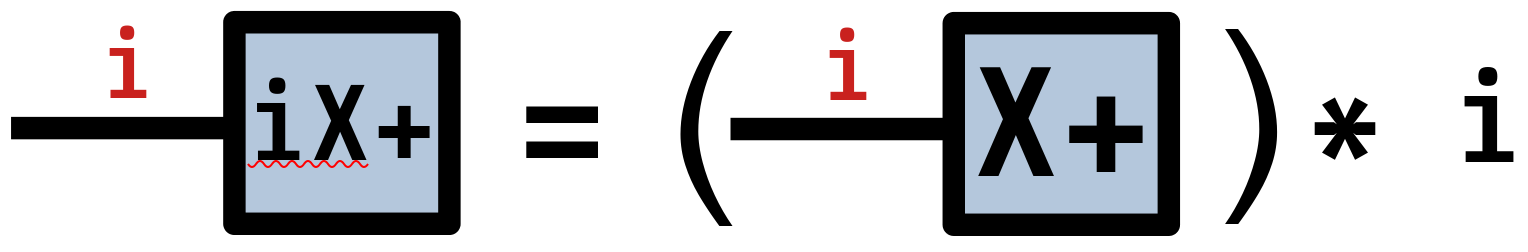
\includegraphics[width=1.0\textwidth]{
  slides/assets/iXp.png
}
\end{onlyenv}

\end{column}

\end{columns}

\end{frame}
